% !TEX root = ../../main.tex

\section{Case studies for the use of 
microcalorimetry combined with adsorption experiments}

\subsection{Comparison between enthalpies of adsorption measured
	through the direct and indirect method}

In order to ascertain the strengths and weaknesses of the isosteric 
and calorimetric method of measuring the enthalpy of adsorption, 
a sample of UiO-66(Zr) previously used for a study of 
carbon dioxide~\cite{wiersumEvaluationUiO66GasBased2011} adsorption
was also measured using microcalorimetry.
Two previous isotherms were recorded through gravimetry at \SI{303}{\kelvin} and
\SI{323}{\kelvin} respectively and the new isotherm was measured in the 
calorimeter at \SI{303}{\kelvin}. The complete set of isotherms can
be found in \autoref{calo:fig:uioisostericiso}.
The two isotherms measured at \SI{303}{\kelvin} are nearly identical, 
ensuring that the both adsorption apparatus are working as intended.
The isosteric enthalpy of adsorption is calculated from the two isotherms
at different temperatures, either using an interpolation method, or through
initial fitting of a virial model (\autoref{pyg:models:virial}).
The values are then adjusted according to \autoref{calo:eqn:adj}.
Calculated and measured values for the enthalpy of adsorption are overlaid
in \autoref{calo:fig:uioisostericheat} as a function of amount adsorbed.

\begin{figure}[htb]
	\centering

	\begin{subfigure}[b]{.5\textwidth}
		\centering
		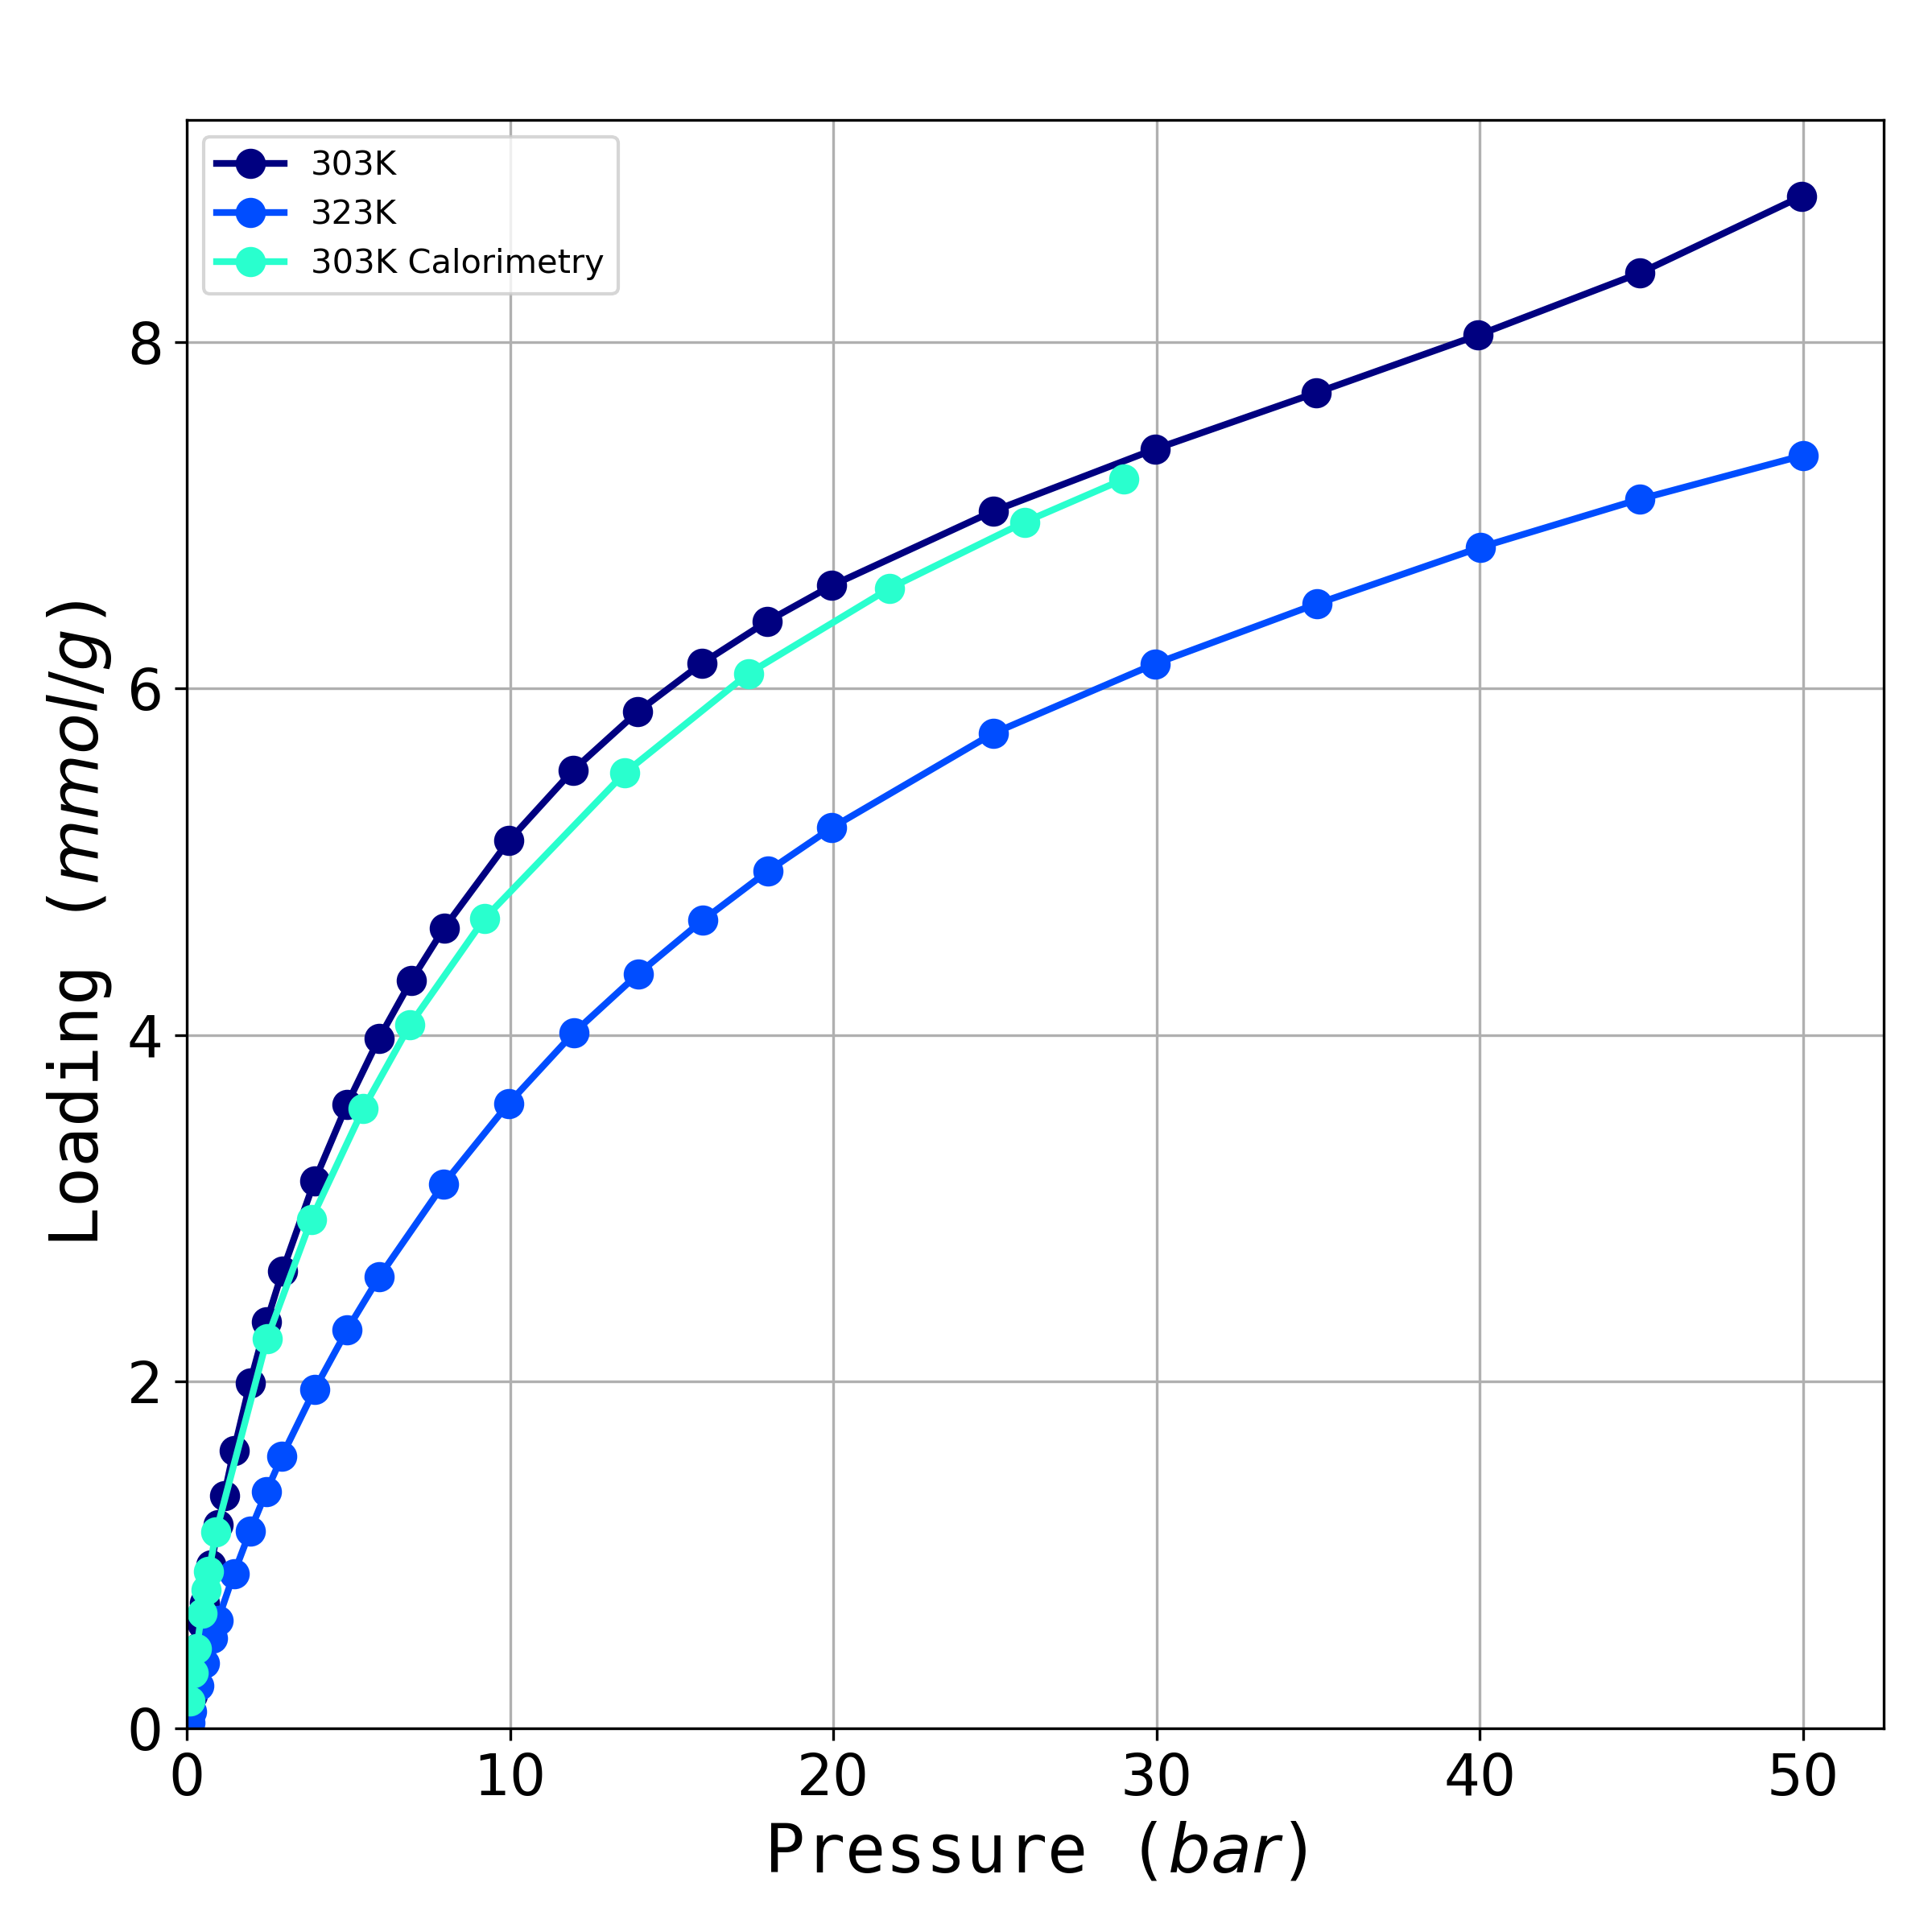
\includegraphics[width=.8\linewidth]{uio/uio-isosteric-iso}
		\caption{}%
		\label{calo:fig:uioisostericiso}
	\end{subfigure}%
	\begin{subfigure}[b]{.5\textwidth}
		\centering
		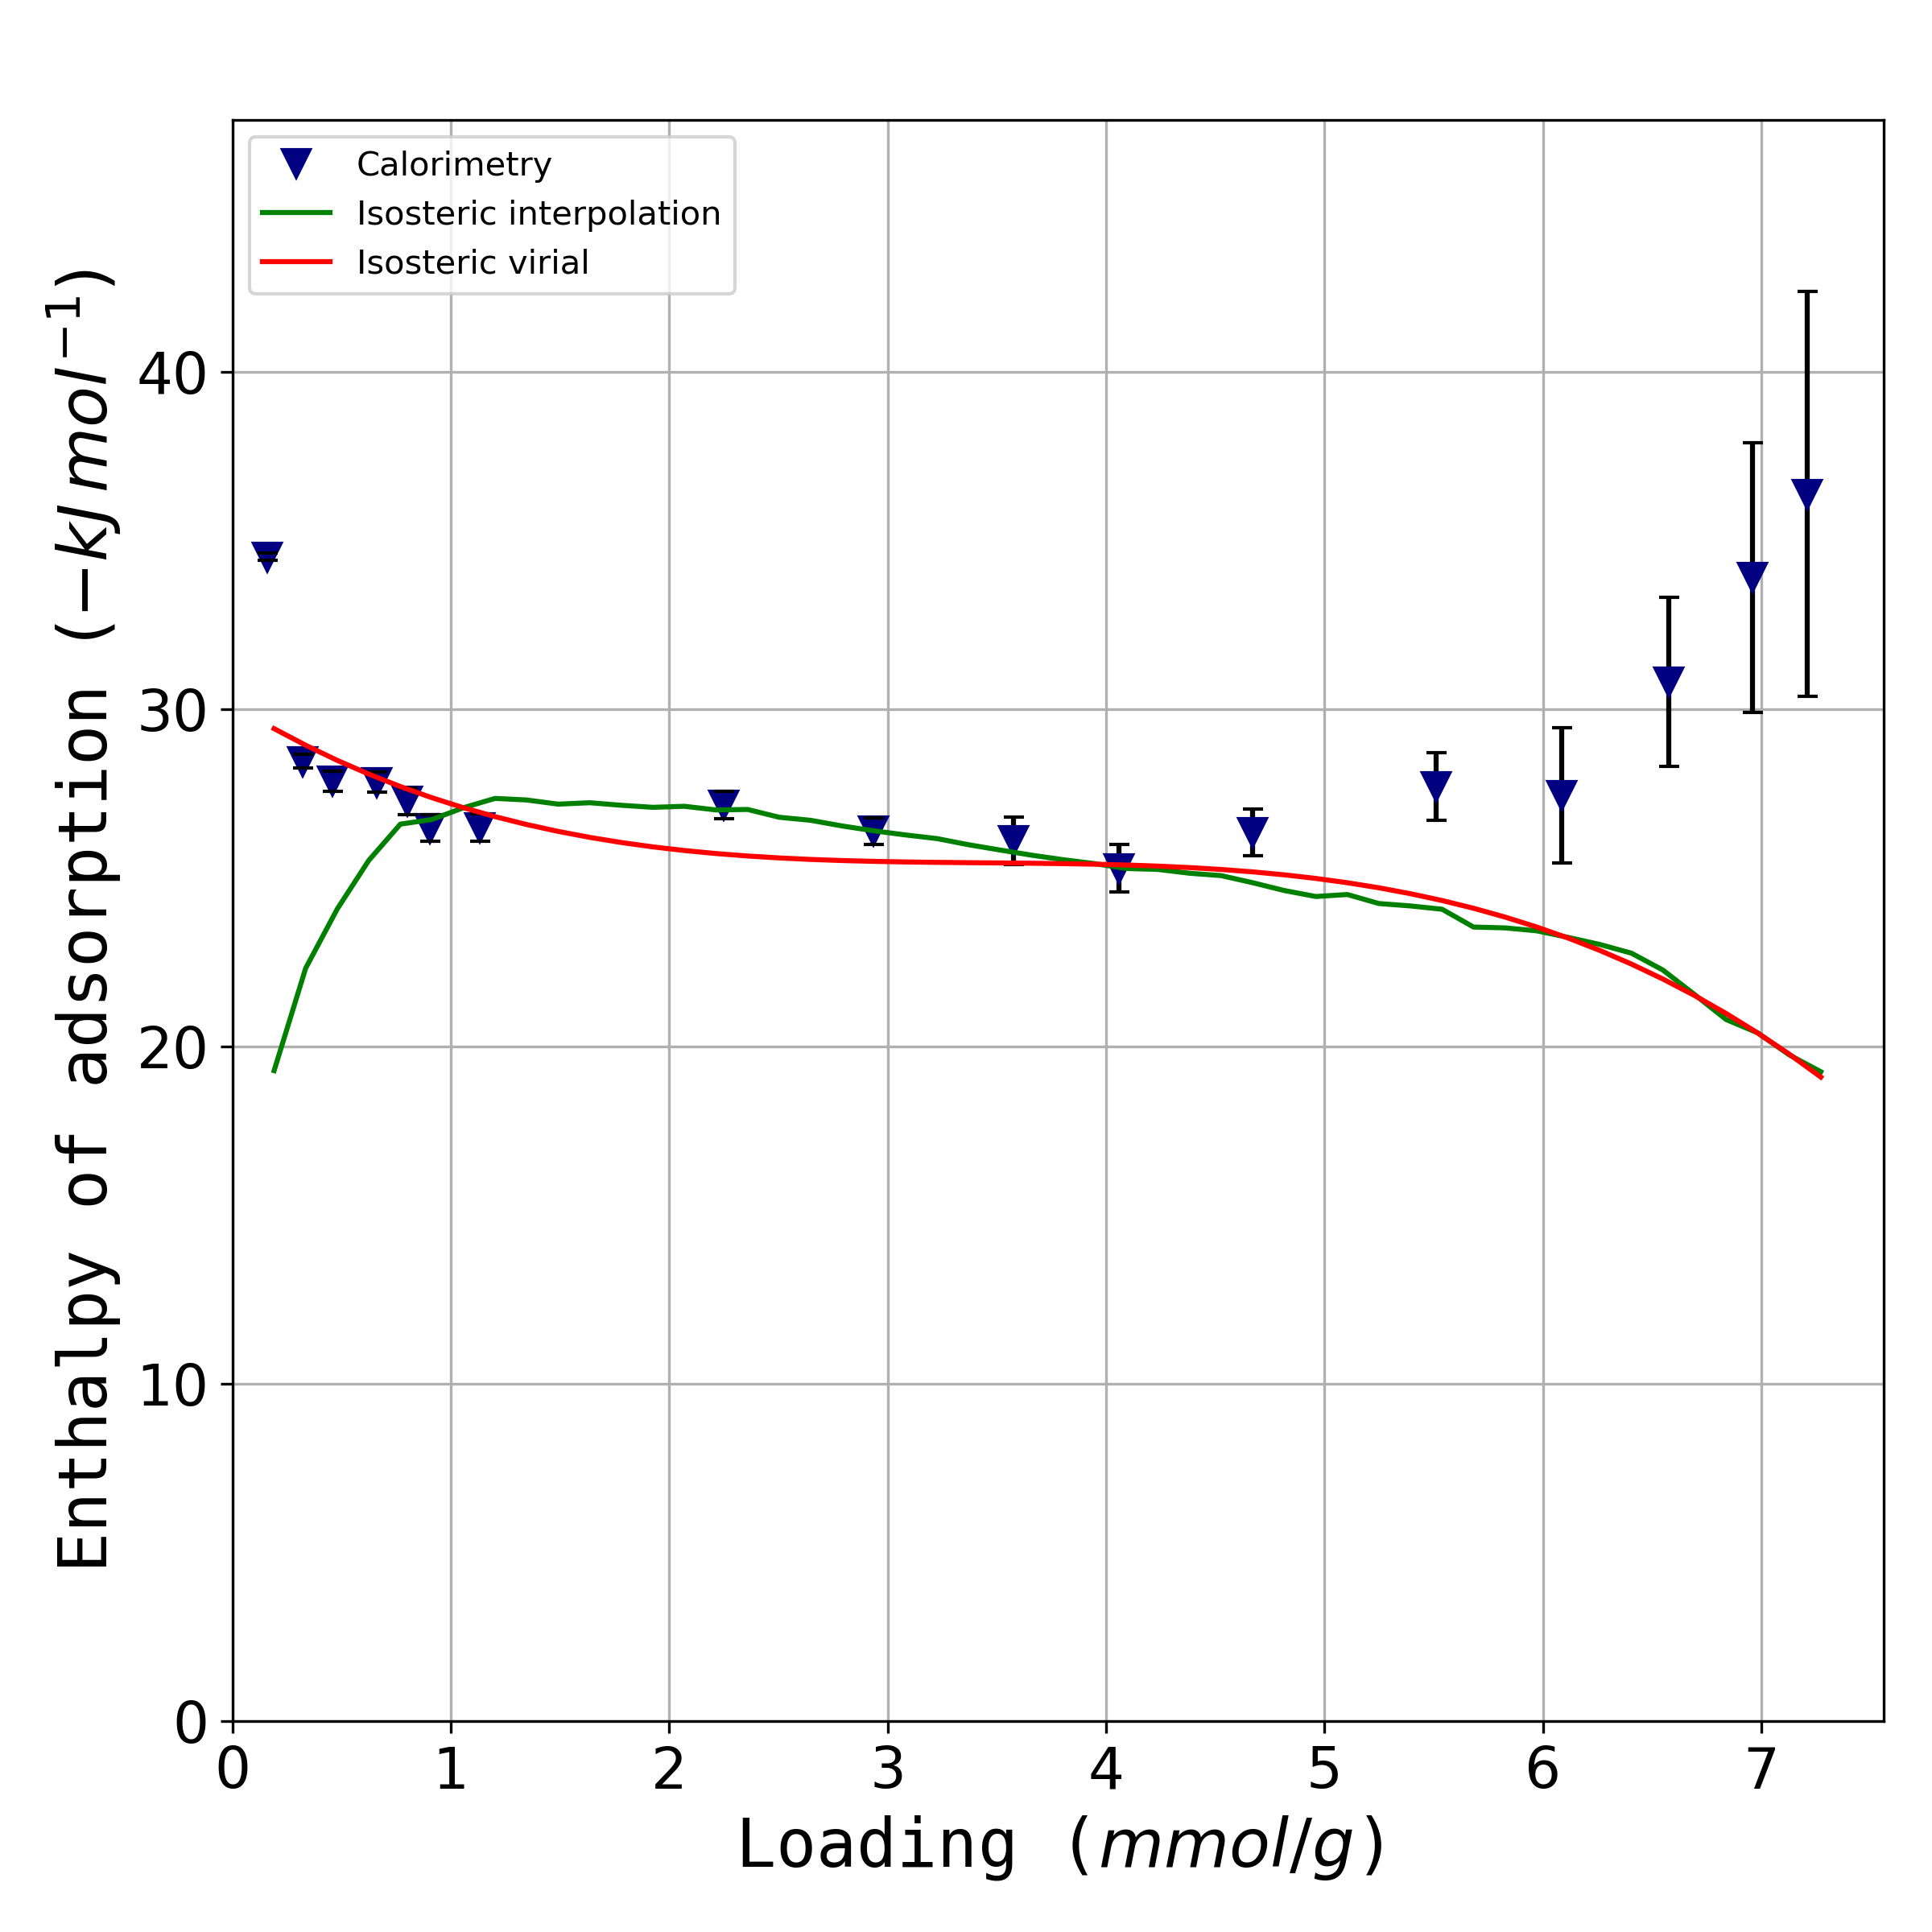
\includegraphics[width=.8\linewidth]{uio/uio-isosteric-heat}
		\caption{}%
		\label{calo:fig:uioisostericheat}
	\end{subfigure}
	\caption{(\protect\subref{calo:fig:uioisostericiso})
		The gravimetric isotherms (red and blue) used for isosteric enthalpy
		calculation and the manometric isotherm measured in the calorimeter (black).
		(\protect\subref{calo:fig:uioisostericheat}) Calculated
		isosteric enthalpy using an interpolation (blue line) and a
		virial fit (red line) of the gravimetric isotherms together with
		the directly measured differential enthalpy of adsorption (blue triangles)}%
	\label{calo:fig:uioisosteric}

\end{figure}

When comparing the differential enthalpy of adsorption measured through
calorimetry to the isosteric enthalpy obtained through interpolation, 
a good overlap can be seen for the most part, but the two values
diverge at low loadings and near complete coverage. 
At low loading the small errors in pressure measurement introduce
large errors in the isosteric enthalpy. By using the model-fitted 
isotherms instead, a better agreement can be achieved. However, the 
virial model still cannot account for the presence of active sites in the 
MOF, as seen in the discrepancy of the first adsorption point.
The calorimetric measurement is therefore more suited to the low pressure
range. At higher loadings, where the isotherm reaches a plateau and
the change in adsorbed amount is small between each adsorbate
insertion, errors are introduced in the enthalpy of adsorption 
calculation from the small adsorbed amounts, as can be seen from the
extent of the error bars in \autoref{calo:fig:uioisostericheat}.
Here, the indirect calculation provides the more accurate results.
As such, the two techniques can be thought of as complementary.

\subsection{An example dataset on a reference material}

A sample of microporous carbon, Takeda 5A (\autoref{appx:synthesis:takeda})
was used as a reference material to exemplify the type of information
that can be obtained through the combined manometric and 
calorimetric method. Pure gas adsorption data has been recorded at 
\SI{303}{\kelvin} using \ce{N2}, \ce{CO}, \ce{CO2}, \ce{CH4}, \ce{C2H6},
\ce{C3H6} and \ce{C3H8} as probes. The complete dataset can be seen 
in \autoref{calo:fig:takeda-dataset}, with the corresponding differential 
enthalpy curves presented in \autoref{calo:fig:takeda-enthalpy}.

\begin{figure}[ht]

	\centering
	\begin{subfigure}[b]{.45\textwidth}
		\centering
		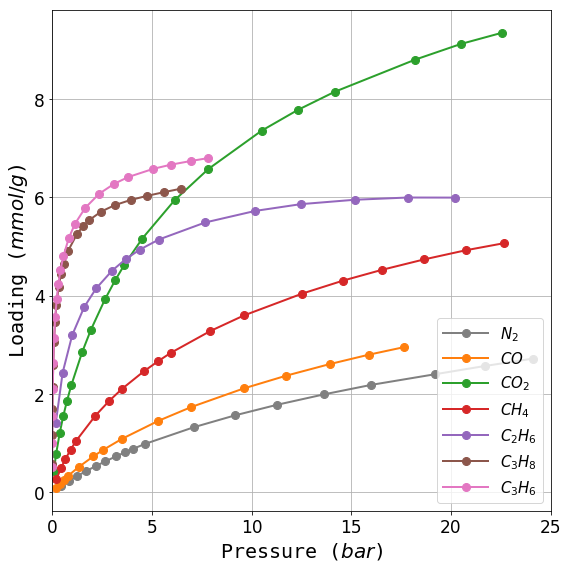
\includegraphics[width=\linewidth]{takeda/takeda-dataset}
		\caption{}%
		\label{calo:fig:takeda-dataset}
	\end{subfigure}%
	\quad
	\begin{subfigure}[b]{.45\textwidth}
		\centering
		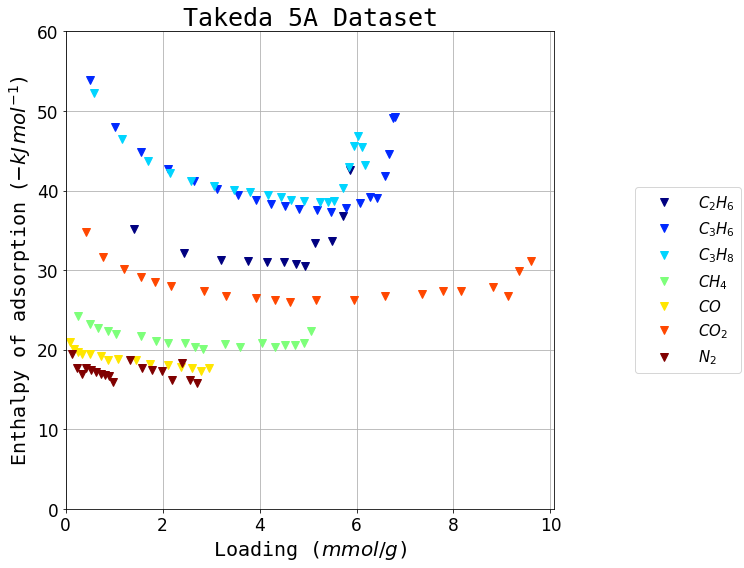
\includegraphics[width=\linewidth]{takeda/takeda-enthalpy}
		\caption{}%
		\label{calo:fig:takeda-enthalpy}
	\end{subfigure}
	\caption{Recorded data on the Takeda 5A sample, 
		(\protect\subref{calo:fig:takeda-dataset}) the
		experimental dataset all recorded gases and 
		(\protect\subref{calo:fig:takeda-enthalpy}) 
		corresponding differential enthalpy.}%
	\label{calo:fig:takeda-data}

\end{figure}

It should first be highlighted that the isotherms can be split into 
two adsorption regimes: subcritical, as is the case for carbon
dioxide and all hydrocarbons except methane, and supercritical,
as is the case for nitrogen, carbon monoxide and methane.
Supercritical gasses do not have any distinction between the 
gaseous and liquid phase, therefore the density of the adsorbed phase
cannot be likened to that of a corresponding liquid. The enthalpy
of vaporisation of such a fluid in this regime is necessarily 0.
However, in-depth studies of supercritical 
isotherms~\cite{doAdsorptionSupercriticalFluids2003} have shown that
the density of the adsorbed phase is highly dependent on the surface 
area of the material. As the interactions in this regime are essentially
restricted to guest-host interactions, the density can can approach that
of a liquid in highly microporous and strong pore field gradient materials.

Nitrogen and carbon monoxide are similar in their adsorption behaviour,
with a nearly linear isotherm and low capacities.
The enthalpy curves are also an indication of non-specific 
interactions with the surface, as the enthalpy of adsorption
is nearly constant throughout the entire loading range.
Carbon dioxide has the highest loading capacity of the entire dataset, likely
due to a combination of a small molecule size and interactions with 
the carbon pore walls. The enthalpy curve shows a higher energy of 
adsorption at low loading by \SIrange{5}{10}{\kilo\joule\per\mole}, 
corresponding to adsorption on a slightly heterogeneous surface.
The adsorption of hydrocarbons takes place in accordance to their size, with
both the initial slope and the enthalpy of adsorption increasing linearly
as a function of the carbon number. Each methyl group is seen 
to contribute, on average, with around \SIrange{10}{15}{\kilo\joule\per\mole}
to the mean enthalpy of adsorption~\cite{denayerChromatographicStudyAdsorption1998}.
When it comes to saturated versus unsaturated hydrocarbons, propylene is 
seen to have a higher capacity than propane. As the enthalpy of 
adsorption is identical at low loading, specific interactions with the 
\(\pi\) electrons of the double bond are unlikely, with packing effects 
from the smaller kinetic diameter of propylene as a more plausible
explanation.

Two parameters can be useful in characterising the local pore environment
before guest-guest interactions come into effect: the Henry constant at
low loadings as well as the initial differential enthalpy of adsorption. 
Here, the initial Henry's constant is calculated by fitting a virial model 
to the isotherm, then taking the limit of the function at zero loading. 

The initial enthalpy of adsorption can be determined from calorimetric 
methods simply by taking the value of the first measured point.
However, this procedure is susceptible to large errors, particularly
if the isotherm has no points in the low coverage region. An alternative
is to take an average of all recorded points, a method which assumes
a homogenous surface. \citet{myersThermodynamicsAdsorptionPorous2002},
has suggested that the enthalpy curve follows a polynomial model, similar
to a virial isotherm.
In this work, an empirical method is used where the enthalpy curve
is treated as a compound contribution from guest-host interaction,
guest-guest attraction and repulsion, the factors of which are determined
using a minimization algorithm. Adsorbate-adsorbate interaction is 
represented as a logistic function, which can account for both 
a heterogeneous surface and a micropore filling step. Power functions
are used for both attraction and repulsion factors. An example of 
an enthalpy curve fitted with this method can be seen 
in \autoref{calo:fig:takeda-enth-fit}

\begin{figure}[ht]

	\centering
	\begin{subfigure}[b]{.5\textwidth}
		\centering
		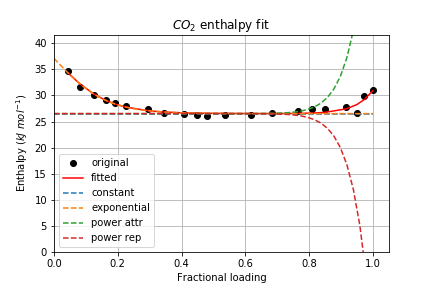
\includegraphics[width=.95\linewidth]{takeda/takeda-enthalpy-fit}
		\caption{}%
		\label{calo:fig:takeda-enth-fit}
	\end{subfigure}%
	\begin{subfigure}[b]{.5\textwidth}
		\centering
		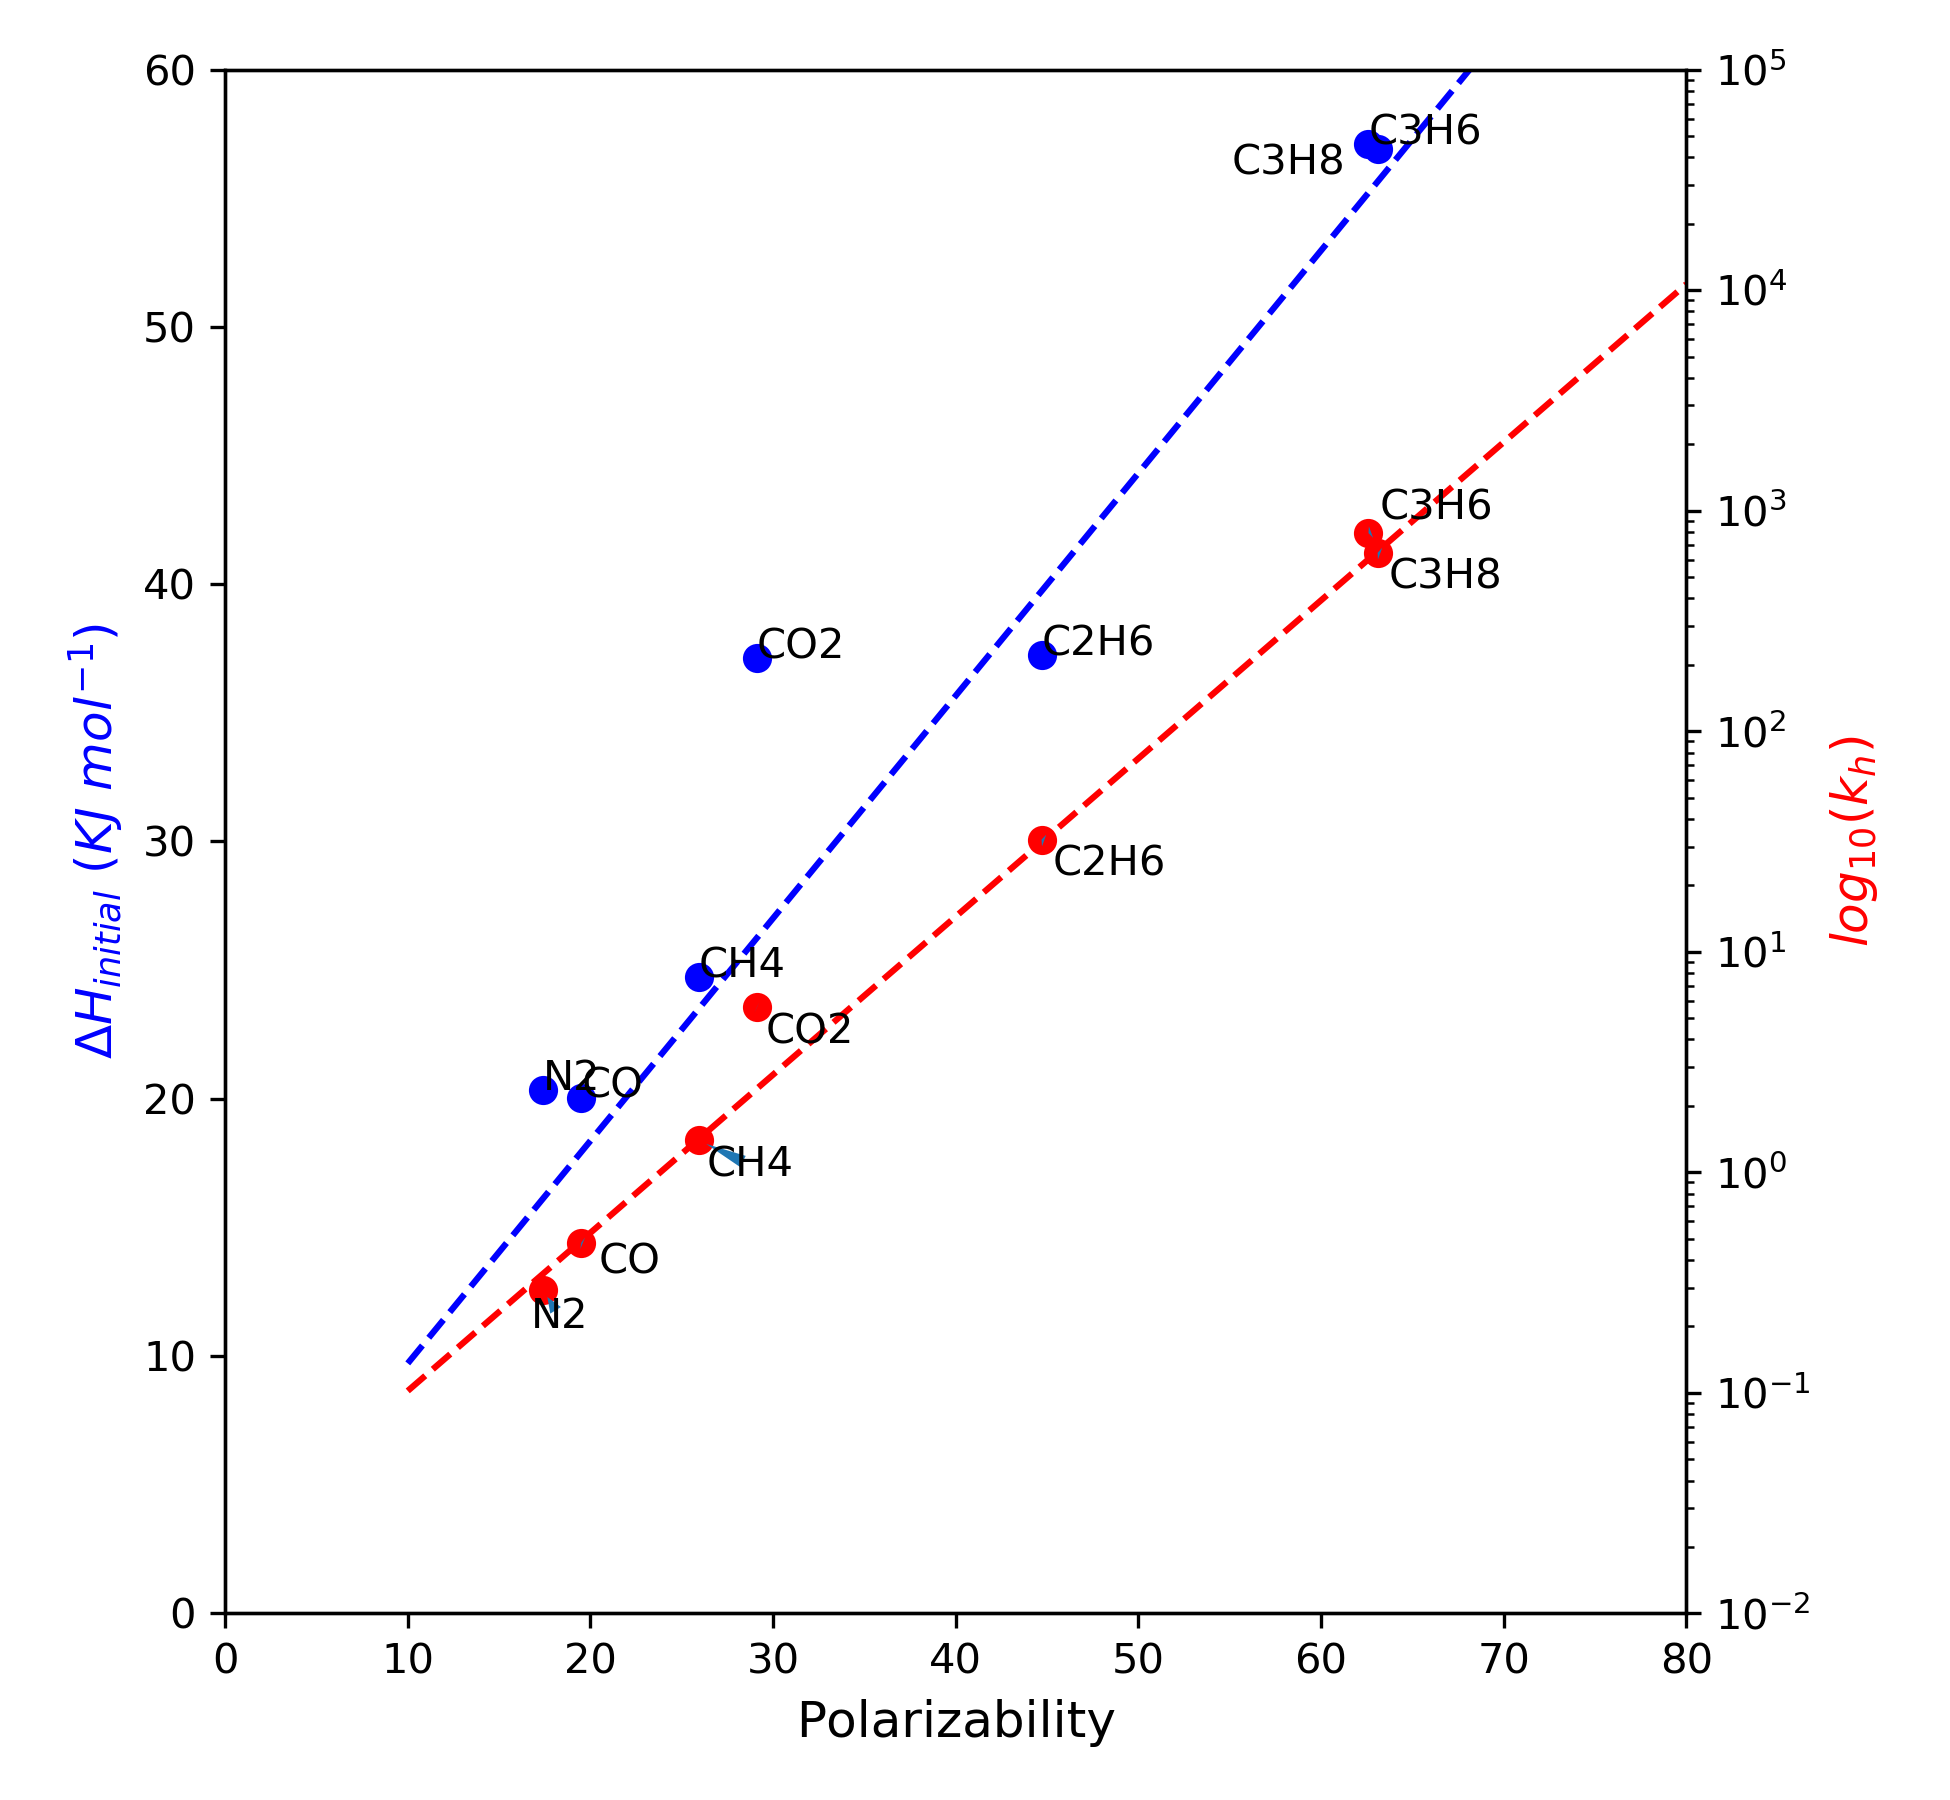
\includegraphics[width=.8\linewidth]{takeda/takeda-enth-henry}
		\caption{}%
		\label{calo:fig:takeda-trends}
	\end{subfigure}
	\caption{Takeda 5A dataset processing: (\protect\subref{calo:fig:takeda-enth-fit})
	 an example of the empirical enthalpy fit model and (\protect\subref{calo:fig:takeda-trends}) the calculated
		trends for initial heat of adsorption and Henry's constant}%
	\label{calo:fig:takeda-analysis}

\end{figure}

A useful method of displaying the two parameters can be to plot them
as a function of the polarizability of the probe, as in
\autoref{calo:fig:takeda-trends}. Both parameters follow a linear
trend, which suggests that the interactions between those guests and the
pore walls are mostly due to non-specific interactions with the field
gradient of the pore. Carbon dioxide has a higher enthalpy
of adsorption than the baseline, which can be ascribed to the contribution 
from its quadrupole moment. There is almost a complete overlap between 
propane and propylene, confirming that the unsaturated double bond does not
interact in a specific way with the carbon surface.

% !TEX root = ../../main.tex

\subsection{A study on a novel MOF}

With the methods of characterisation through calorimetry
outlined on a reference material, a similar study on a 
\gls{MOF} sample can be performed. The aim is to screen for 
potentially interesting features for use in gas 
storage and separation.

\subsubsection{Material}

Zr Fumarate, also known as MOF-801, is a fumaric 
acid analogue of the well-known UiO-66(Zr) 
framework~\cite{wissmannModulatedSynthesisZrfumarate2012}.
Its structure is similar to that of UiO-66, although 
the smaller non-linear linker leads to a lowering of 
symmetry and a slight tilting in the Zr-O clusters,
as depicted in \autoref{calo:fig:zrfum-structure}.
The \gls{MOF} is synthesised using the modulated synthesis method and 
formic acid as the modulator to increase the crystalinity of the
material. Indeed, when not using this approach, the resulting
material is nearly amorphous~\cite{zahnInsightMechanismModulated2014}.
In this study the sample was synthesised according to the procedure 
detailed in \autoref{appx:synthesis:zrformate}.

\begin{figure}[htb]
    \centering
    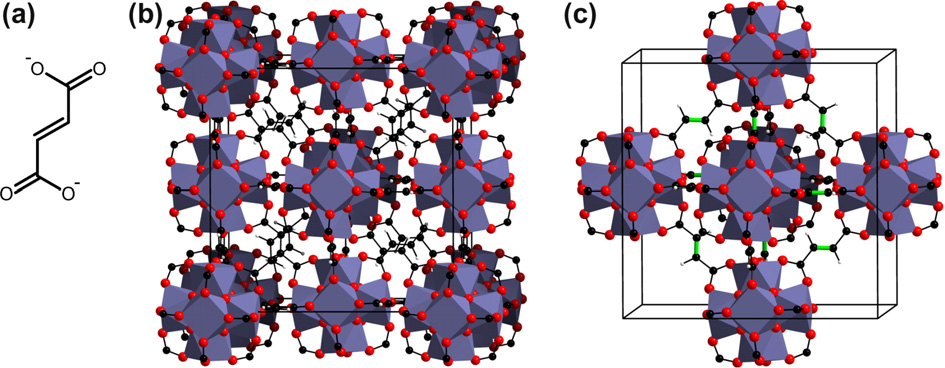
\includegraphics[width=0.8\textwidth]{zrfum/structure}%
    \caption{(a) The fumarate linker used in the Zr Fumarate
    \gls{MOF}, an ionic form of \textit{trans}-butenedioic acid and
    (b) and (c) the structural model of the \gls{MOF}. Illustration
    adapted from~\citet{wissmannModulatedSynthesisZrfumarate2012}.}%
    \label{calo:fig:zrfum-structure}
\end{figure}

Zr Fumarate has recently been the subject of interest due to its
high water stability~\cite{zahnWaterbornZrbasedPorous2015}, 
as well as its potential to be synthesised through green synthesis
routes~\cite{reinschFacileGreenRoute2016} or direct
monolith formation with a gel approach~\cite{buekenGelbasedMorphologicalDesign2017}.
Furthermore, the material has a remarkably steep water adsorption
behaviour at low pressure~\cite{furukawaWaterAdsorptionPorous2014},
which has led to its possible application as a water scavenger 
membrane~\cite{baeTransparentMetalOrganic2016} or in a water 
harvesting device which would capture water from air in low relative
humidity environments such as the desert. While initial 
attempts~\cite{kimWaterHarvestingAir2017} were criticised for
overpromising performance, more recent modifications to such 
a system have addressed some of these 
concerns~\cite{kimAdsorptionbasedAtmosphericWater2018}.
The low relative pressure of water adsorption has highlighted
the contribution of defects~\cite{choiRoleStructuralDefects2018} in 
shifting the adsorption isotherm, an effect arising from cooperative
interactions and initial clustering of water molecules on defect
sites~\cite{vandichelWaterCoordinationDehydration2016}.

As the properties of the \gls{MOF} diverge from the ideal properties
indicated by the structure, an experimental study to test for the adsorption
or separation of other molecules may reveal unexpected 
applications.

\subsubsection{Results}

Adsorption isotherms of nine probe gasses were recorded at 
\SI{303}{\kelvin} through combined manometry and microcalorimetry
as described in \autoref{calo:method:calo}. The complete 
dataset can be seen in \autoref{calo:fig:zrfum-data}.
The results are remarkably similar to the Takeda 5A carbon, with 
very similar trends visible. All isotherms are somewhat 
shifted downwards, which suggests less interaction with the 
pore walls and a lower total pore volume. The enthalpies of 
adsorption are on average lower by \SIrange{5}{7}{\kilo\joule\per\mol},
confirming that the guest-host attraction is overall lower than
in the carbon. Argon, oxygen and nitrogen isotherms are essentially
following Henry's law in the measured pressure range, with nearly constant
enthalpies of adsorption. Carbon dioxide adsorption enthalpy is seen to take
place on specific sites at the start of the isotherm, then
decreasing until around \SI{25}{{\kilo\joule\per\mol}}. Cooperative
interactions take over afterwards, slowly increasing the enthalpy 
of adsorption.

\begin{figure}[htb]
    \centering

	\begin{subfigure}[b]{.45\textwidth}
        \centering
        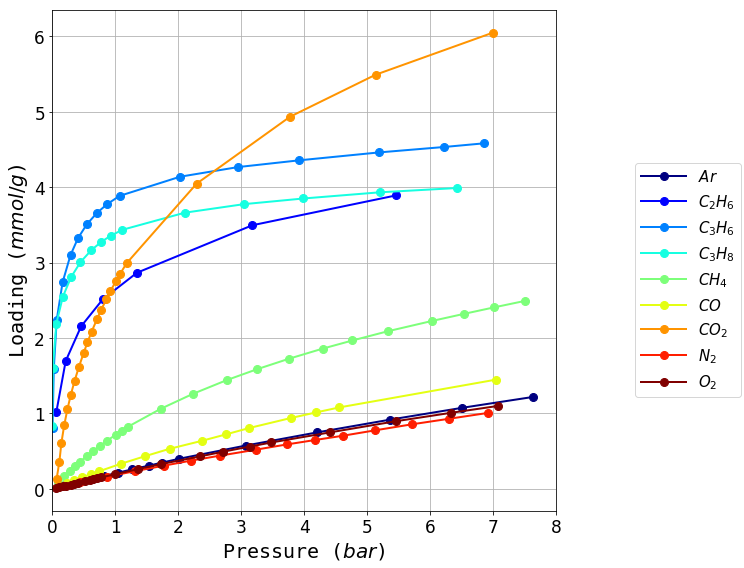
\includegraphics[width=\linewidth]{zrfum/zrfum-dataset}
        \caption{}%
        \label{calo:fig:zrfum-dataset}
    \end{subfigure}%
	\quad
	\begin{subfigure}[b]{.45\textwidth}
        \centering
        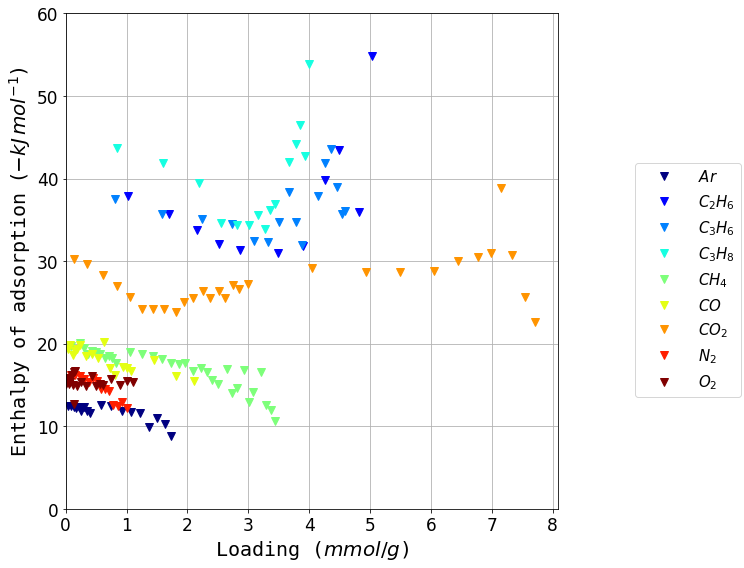
\includegraphics[width=\linewidth]{zrfum/zrfum-enthalpy}
        \caption{}%
        \label{calo:fig:zrfum-enthalpy}
    \end{subfigure}
    \caption{(a) The experimental isotherms of all recorded gases and
    (b) the corresponding enthalpy curves.}%
    \label{calo:fig:zrfum-data}

\end{figure}

The propane and propylene isotherms also show a higher total
loading for propylene at the plateau. However, the enthalpy
curve suggests a higher adsorption enthalpy of propane at lower
loading. A similar plot for initial Henry's constant and
enthalpy of adsorption at zero loading, in \autoref{calo:fig:zrfum-trends},
confirms this trend, with propylene showing a decreased value
in both parameters. As propane still lies on the trendline generated
by unsaturated hydrocarbons, it does not seem that it possesses any
increased specific interactions with the \gls{MOF} surface. Instead, 
the expected values for propylene are lower than those of its
saturated counterpart. It should be pointed out that the
slope of the trendline is lower than that of the Takeda 5A. This slope 
can be thought of as a measure of the non-specific interaction strength
of the adsorbate surface and described through a field gradient,
influenced by the chemistry and size of the pore.

\begin{figure}[htb]
    \centering
    
    \begin{subfigure}[b]{0.5\textwidth}
        \centering
        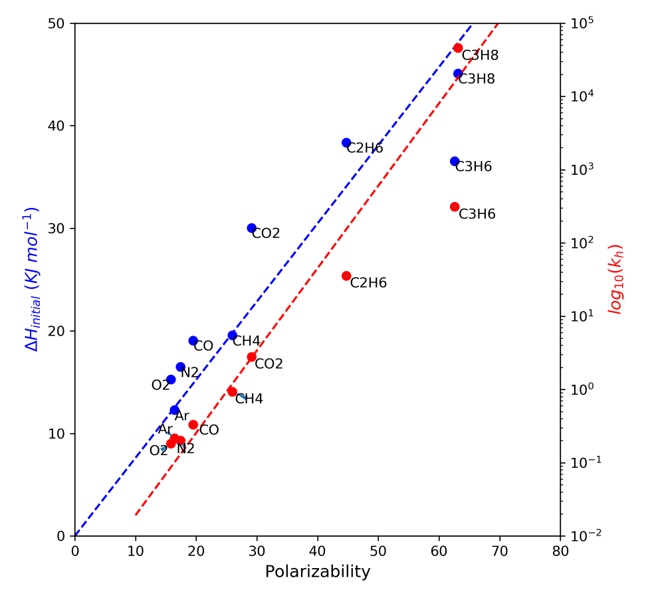
\includegraphics[width=\linewidth]{zrfum/zrfum-enth-henry}
        \caption{}%
        \label{calo:fig:zrfum-trends}
    \end{subfigure}%
    \begin{subfigure}[b]{0.45\textwidth}
        \centering
        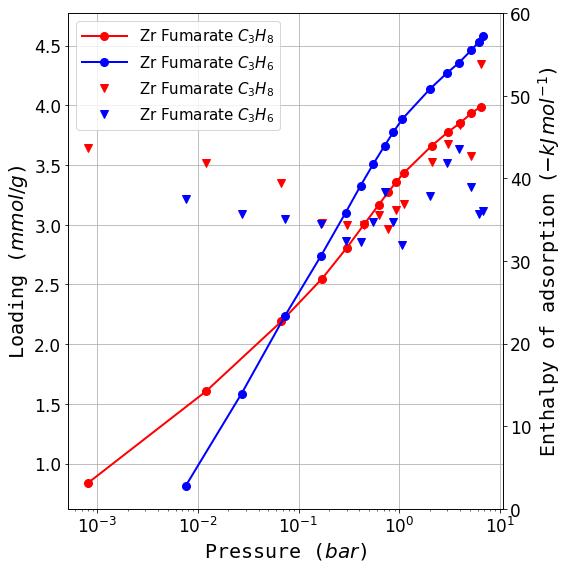
\includegraphics[width=\linewidth]{zrfum/zrfum-close}
        \caption{}%
        \label{calo:fig:zrfum-close}
    \end{subfigure}%
    \caption{(a) Calculated trends for initial heat of adsorption (red) and 
    Henry's constant (blue) as a function of polarizability for 
    Zr Fumarate. The dotted lines are best fit lines to 
    the series of unsaturated hydrocarbons. (b) Logarithmic form of the 
    propane and propylene isotherms.}%
    \label{calo:fig:zrfum-analysis}

\end{figure}

When examining the low pressure region of the two isotherms 
(\autoref{calo:fig:zrfum-close}) a preference for propane over
propylene can be observed, which is the source of the anomaly
in the polarizability graph. The isotherms then ``cross over'' 
at higher pressures.
This behaviour has been reproduced by measuring the same 
isotherms with a commercial apparatus, which can be found 
in \autoref{appx:calo}.
A higher selectivity for propylene adsorption is not uncommon
in materials with open metal sites which can interact with 
the \(\pi\) electrons of the 
molecule~\cite{rubesAdsorptionPropanePropylene2013}.
Furthermore, \glspl{MOF} with pore sizes perfectly tuned for kinetically
selective adsorption of propylene over propane have been shown 
to exist~\cite{leeKineticSeparationPropene2011}. However,
the preference for propane in this material is surprising.
The effect itself is unlikely to arise from simple diffusion
effects~\cite{granatoDiffusionPropanePropylene2010}, although
it has been shown~\cite{combarizaPropanePropyleneDiffusion2009}
that pore windows can dominate diffusion behaviour. A contribution
from framework defects is also be likely, as the 
crystal structure calculated pore volume is 40\% of the total
volume as determined from the propane adsorption isotherm.
Thermogravimetry and water adsorption experiments, available in 
\autoref{appx:calo}, both confirm the presence of defects in the 
material structure.

\begin{figure}[htb]
    \centering
    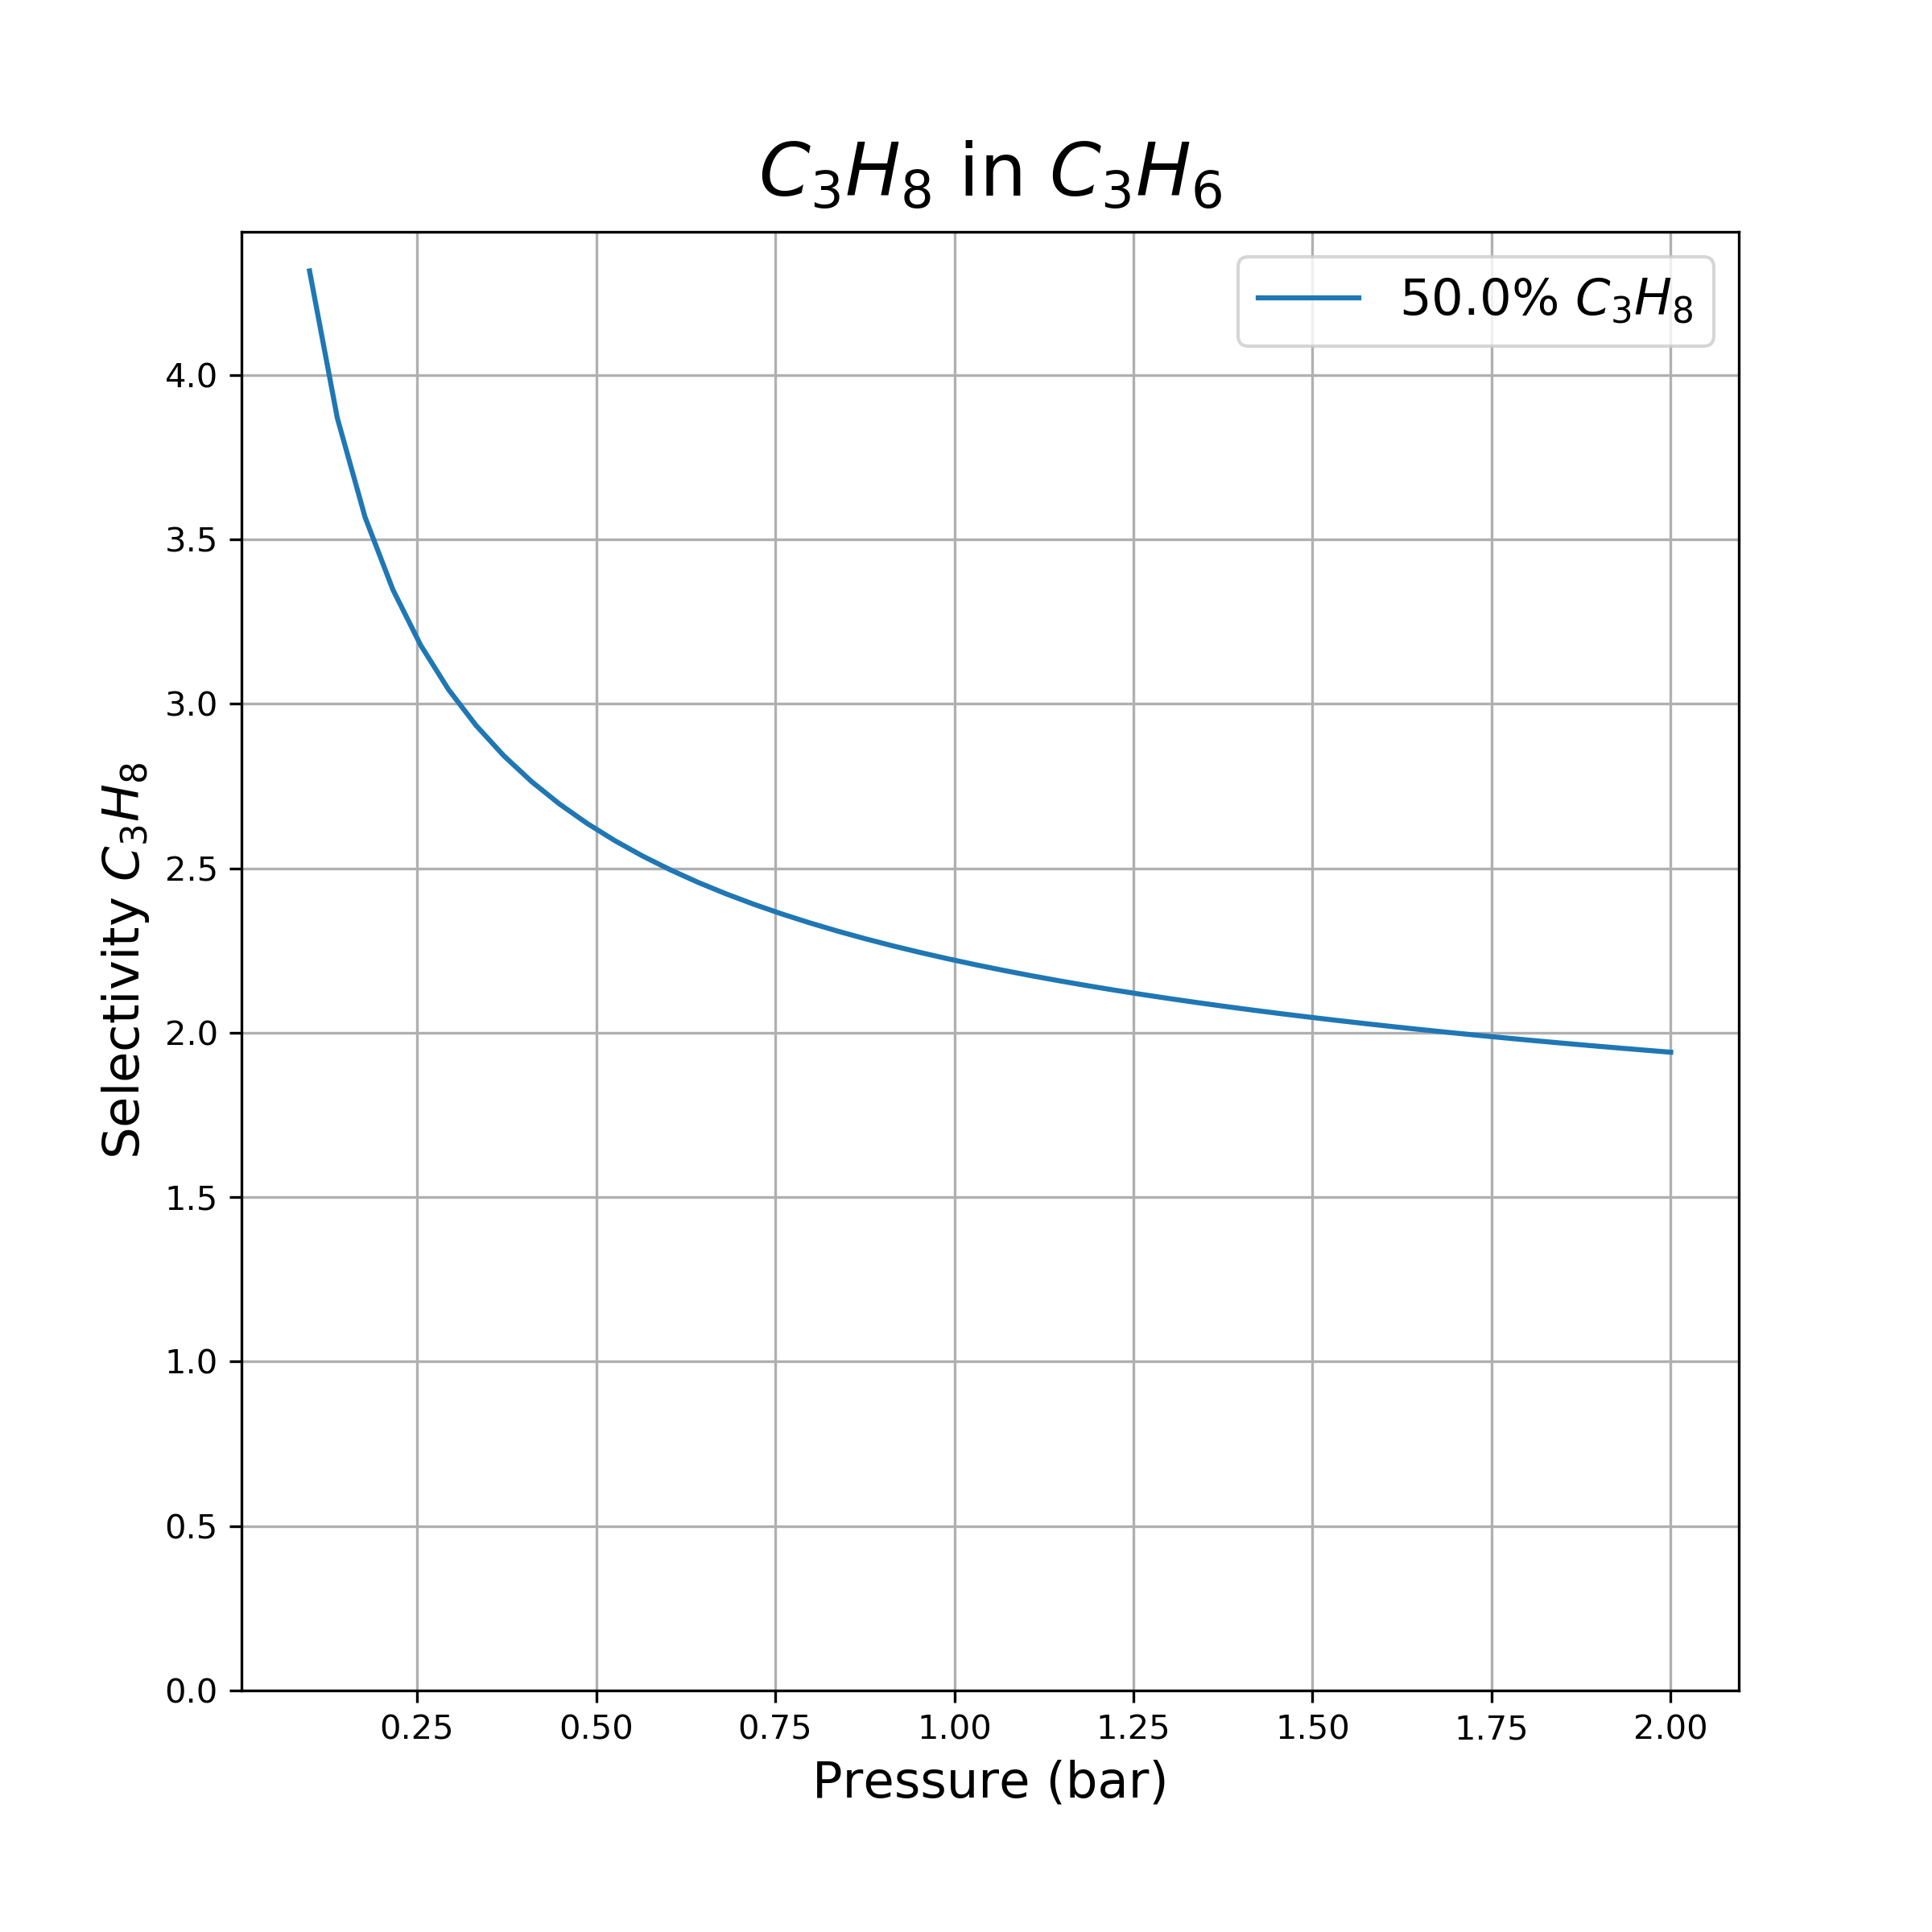
\includegraphics[width=0.5\linewidth]{zrfum/zrfum-iast}
    \caption{IAST simulation of an equimolar mixture of 
    propane and propylene on Zr Fumarate}%
    \label{calo:fig:zrfum-iast}

\end{figure}

To observe the impact on separation efficiency, the two isotherms 
are fitted with the best conforming model, in this case
double site Langmuir, and \gls{IAST} simulations of an equimolar mixture
of propane and propylene are carried out as seen in 
\autoref{calo:fig:zrfum-iast}. A selectivity of 4--2 for 
propane is predicted by \gls{IAST}, which may be of interest in 
large-scale processes, as even a small separation factor 
improvement may yield large energy savings.

In this case, direct measurement of the differential enthalpy of 
adsorption has highlighted several behaviours unique to this 
\gls{MOF}. However, in order to understand the source and mechanism
of this effect, further study is recommended. Molecular 
simulation of adsorption isotherms can reveal whether 
the process is kinetically or thermodynamically controlled, as well
as give an indication of the contribution of defect sites to the
guest-host molecular interactions.
Concomitantly, breakthrough experiments in an adsorbent column of 
the \gls{MOF} or binary adsorption experiments can confirm whether the 
effect holds when a mixture of the two hydrocarbons is present.
